% Source PDF page 471 (printed p. 457)
\section{无约束最小化问题}
本章讨论求解无约束优化问题
\begin{equation}
\text{最小化}\quad f(x)\tag{9.1}
\end{equation}
的方法，其中 $f:\R^n\to\R$ 凸且二阶连续可微（因此 $\dom f$ 是开集）。假设问题有解，即存在最优点 $x^\star$。（更准确地说，本章稍后的假设将保证 $x^\star$ 存在且唯一。）用 $p^\star$ 表示最优值 $\inf_xf(x)=f(x^\star)$。

由于 $f$ 可微且凸，点 $x^\star$ 最优的充要条件是
\begin{equation}
\nabla f(x^\star)=0\tag{9.2}
\end{equation}
（见§4.2.3）。因此，求解无约束最小化问题（9.1），等同于求解（9.2），即一组含 $n$ 个变量 $x_1,\ldots,x_n$ 的 $n$ 个方程。少数特殊情形下，可以解析求解最优性方程（9.2），从而得到（9.1）的解；但通常必须用迭代算法。这里指算法计算一列点 $x^{(0)},x^{(1)},\ldots\in\dom f$，使 $k\to\infty$ 时 $f(x^{(k)})\to p^\star$。这样的点列称为问题（9.1）的\emph{极小化序列}。当 $f(x^{(k)})-p^\star\le\epsilon$ 时算法终止，其中 $\epsilon>0$ 为指定容差。

\subsubsection*{初始点与下水平集}
本章的方法需要适当初始点 $x^{(0)}$。初始点必须属于 $\dom f$，而且下水平集
\begin{equation}
S=\{x\in\dom f\mid f(x)\le f(x^{(0)})\}\tag{9.3}
\end{equation}
必须闭。若函数 $f$ 闭，即所有下水平集闭（见§A.3.3），则任意 $x^{(0)}\in\dom f$ 都满足此条件。定义域为 $\R^n$ 的连续函数都是闭函数。

% Source PDF page 472 (printed p. 458)
因此，若 $\dom f=\R^n$，任意 $x^{(0)}$ 都满足初始下水平集条件。另一类重要闭函数是具有开定义域的连续函数，且当 $x$ 趋近 $\operatorname{bd}\dom f$ 时 $f(x)$ 趋于无穷大。

\subsection{例子}
\subsubsection*{二次最小化与最小二乘}
一般凸二次最小化问题形式为
\begin{equation}
\text{最小化}\quad(1/2)x^\T Px+q^\T x+r,\tag{9.4}
\end{equation}
其中 $P\in\mathbf S_+^n$、$q\in\R^n$、$r\in\R$。可通过最优性条件 $Px^\star+q=0$ 求解，这是线性方程组。当 $P\succ0$ 时，解唯一，为 $x^\star=-P^{-1}q$。更一般地，当 $P$ 非正定时，$Px^\star=-q$ 的任意解都是（9.4）的最优解；若该方程无解，则（9.4）无下界（见习题9.1）。能够解析求解二次最小化问题（9.4），是牛顿法的基础；牛顿法是强有力的无约束最小化方法，在§9.5介绍。

二次最小化一个极常见的特殊情形是最小二乘问题
\[
\text{最小化}\quad
\norm{Ax-b}_2^2=x^\T(A^\T A)x-2(A^\T b)^\T x+b^\T b.
\]
其最优性条件
\[
A^\T Ax^\star=A^\T b
\]
称为最小二乘问题的\emph{正规方程}。

\subsubsection*{无约束几何规划}
第二个例子是凸形式的无约束几何规划
\[
\text{最小化}\quad
f(x)=\log\left(\sum_{i=1}^m\exp(a_i^\T x+b_i)\right).
\]
最优性条件为
\[
\nabla f(x^\star)=
\frac1{\sum_{j=1}^m\exp(a_j^\T x^\star+b_j)}
\sum_{i=1}^m\exp(a_i^\T x^\star+b_i)a_i=0.
\]
它通常没有解析解，所以必须采用迭代算法。这个问题的 $\dom f=\R^n$，因此可任选一点作为初始点 $x^{(0)}$。

\subsubsection*{线性不等式的解析中心}
考虑优化问题
\begin{equation}
\text{最小化}\quad
f(x)=-\sum_{i=1}^m\log(b_i-a_i^\T x),\tag{9.5}
\end{equation}

% Source PDF page 473 (printed p. 459)
其中 $f$ 的定义域是开集
\[
\dom f=\{x\mid a_i^\T x<b_i,\ i=1,\ldots,m\}.
\]
该问题的目标函数 $f$ 称为不等式 $a_i^\T x\le b_i$ 的\emph{对数障碍}。问题（9.5）的解若存在，称为这些不等式的\emph{解析中心}。初始点 $x^{(0)}$ 必须满足严格不等式 $a_i^\T x^{(0)}<b_i$，$i=1,\ldots,m$。由于 $f$ 闭，任意这样的点对应的下水平集 $S$ 都闭。

\subsubsection*{线性矩阵不等式的解析中心}
一个密切相关的问题是
\begin{equation}
\text{最小化}\quad f(x)=\log\det F(x)^{-1},\tag{9.6}
\end{equation}
其中 $F:\R^n\to\mathbf S^p$ 仿射，即
\[
F(x)=F_0+x_1F_1+\cdots+x_nF_n,
\]
$F_i\in\mathbf S^p$。这里 $f$ 的定义域为
\[
\dom f=\{x\mid F(x)\succ0\}.
\]
目标函数 $f$ 称为线性矩阵不等式 $F(x)\succeq0$ 的\emph{对数障碍}，其解（若存在）称为该线性矩阵不等式的\emph{解析中心}。初始点 $x^{(0)}$ 必须满足严格线性矩阵不等式 $F(x^{(0)})\succ0$。与前例一样，由于 $f$ 闭，任意这种点的下水平集闭。

\subsection{强凸性及其推论}
本章大部分内容（§9.6除外）假设目标函数在 $S$ 上\emph{强凸}，即存在 $m>0$，使所有 $x\in S$ 都满足
\begin{equation}
\nabla^2 f(x)\succeq mI.\tag{9.7}
\end{equation}
强凸性有几个有趣的推论。对 $x,y\in S$，有
\[
f(y)=f(x)+\nabla f(x)^\T(y-x)
+\tfrac12(y-x)^\T\nabla^2f(z)(y-x),
\]
其中 $z$ 是线段 $[x,y]$ 上的某点。由强凸假设（9.7），右端最后一项至少为 $(m/2)\norm{y-x}_2^2$，所以对所有 $x,y\in S$，
\begin{equation}
f(y)\ge f(x)+\nabla f(x)^\T(y-x)+\frac m2\norm{y-x}_2^2.\tag{9.8}
\end{equation}
当 $m=0$ 时，就得到刻画凸性的基本不等式；$m>0$ 时，得到的 $f(y)$ 下界比单凭凸性得到的更好。

% Source PDF page 474 (printed p. 460)
先说明如何用（9.8）以 $\norm{\nabla f(x)}_2$ 为 $f(x)-p^\star$（即 $x$ 的次优程度）求界。固定 $x$ 后，（9.8）右端是关于 $y$ 的凸二次函数。令关于 $y$ 的梯度为零，可知 $\widetilde y=x-(1/m)\nabla f(x)$ 使右端最小。因此
\[
\begin{aligned}
f(y)&\ge f(x)+\nabla f(x)^\T(y-x)+\frac m2\norm{y-x}_2^2\\
&\ge f(x)+\nabla f(x)^\T(\widetilde y-x)+\frac m2\norm{\widetilde y-x}_2^2\\
&=f(x)-\frac1{2m}\norm{\nabla f(x)}_2^2.
\end{aligned}
\]
由于对任意 $y\in S$ 都成立，故
\begin{equation}
p^\star\ge f(x)-\frac1{2m}\norm{\nabla f(x)}_2^2.\tag{9.9}
\end{equation}
这说明，若某点的梯度很小，该点就接近最优。还可将（9.9）解释为推广最优性条件（9.2）的次优性条件：
\begin{equation}
\norm{\nabla f(x)}_2\le(2m\epsilon)^{1/2}
\ \Longrightarrow\ f(x)-p^\star\le\epsilon.\tag{9.10}
\end{equation}

还能用 $\norm{\nabla f(x)}_2$ 为 $x$ 到任意最优点 $x^\star$ 的距离 $\norm{x-x^\star}_2$ 求界：
\begin{equation}
\norm{x-x^\star}_2\le\frac2m\norm{\nabla f(x)}_2.\tag{9.11}
\end{equation}
在（9.8）中取 $y=x^\star$，有
\[
\begin{aligned}
p^\star=f(x^\star)
&\ge f(x)+\nabla f(x)^\T(x^\star-x)+\frac m2\norm{x^\star-x}_2^2\\
&\ge f(x)-\norm{\nabla f(x)}_2\norm{x^\star-x}_2+\frac m2\norm{x^\star-x}_2^2,
\end{aligned}
\]
第二个不等式利用Cauchy--Schwarz不等式。由于 $p^\star\le f(x)$，必有
\[
-\norm{\nabla f(x)}_2\norm{x^\star-x}_2+\frac m2\norm{x^\star-x}_2^2\le0,
\]
由此得到（9.11）。其一个推论是最优点 $x^\star$ 唯一。

\subsubsection*{$\nabla^2f(x)$ 的上界}
（9.8）意味着包含在 $S$ 中的下水平集有界，特别地，$S$ 本身有界。因此，$\nabla^2f(x)$ 的最大特征值作为 $S$ 上关于 $x$ 的连续函数，在 $S$ 上有上界，即存在常数 $M$，使所有 $x\in S$ 满足
\begin{equation}
\nabla^2f(x)\preceq MI.\tag{9.12}
\end{equation}

% Source PDF page 475 (printed p. 461)
Hessian的这个上界意味着，对于任意 $x,y\in S$，
\begin{equation}
f(y)\le f(x)+\nabla f(x)^\T(y-x)+\frac M2\norm{y-x}_2^2,\tag{9.13}
\end{equation}
它类似于（9.8）。两边对 $y$ 最小化，得到
\begin{equation}
p^\star\le f(x)-\frac1{2M}\norm{\nabla f(x)}_2^2,\tag{9.14}
\end{equation}
对应于（9.9）。

\subsubsection*{下水平集的条件数}
由强凸不等式（9.7）和（9.12），对所有 $x\in S$，
\begin{equation}
mI\preceq\nabla^2f(x)\preceq MI.\tag{9.15}
\end{equation}
比值 $\kappa=M/m$ 因而是矩阵 $\nabla^2f(x)$ 的条件数（最大特征值与最小特征值之比）的上界。还可用 $f$ 的下水平集为（9.15）给出几何解释。

对凸集 $C\subseteq\R^n$，定义其沿方向 $q$（$\norm q_2=1$）的\emph{宽度}为
\[
W(C,q)=\sup_{z\in C}q^\T z-\inf_{z\in C}q^\T z.
\]
$C$ 的最小和最大宽度为
\[
W_{\min}=\inf_{\norm q_2=1}W(C,q),\qquad
W_{\max}=\sup_{\norm q_2=1}W(C,q).
\]
凸集 $C$ 的\emph{条件数}定义为
\[
\operatorname{cond}(C)=\frac{W_{\max}^2}{W_{\min}^2},
\]
即最大宽度与最小宽度之比的平方。$C$ 的条件数衡量其各向异性或偏心程度。条件数小（例如接近1），表示集合在各方向的宽度大致相同，即接近球形；条件数大，则表示某些方向远比其他方向宽。

\begin{origexample}{9.1}
\emph{椭球的条件数。}设椭球
\[
\mathcal E=\{x\mid(x-x_0)^\T A^{-1}(x-x_0)\le1\},
\]
其中 $A\in\mathbf S_{++}^n$。$\mathcal E$ 沿 $q$ 方向的宽度为
\[
\begin{aligned}
\sup_{z\in\mathcal E}q^\T z-\inf_{z\in\mathcal E}q^\T z
&=(\norm{A^{1/2}q}_2+q^\T x_0)-(-\norm{A^{1/2}q}_2+q^\T x_0)\\
&=2\norm{A^{1/2}q}_2.
\end{aligned}
\]

% Source PDF page 476 (printed p. 462)
所以其最小、最大宽度为
\[
W_{\min}=2\lambda_{\min}(A)^{1/2},\qquad
W_{\max}=2\lambda_{\max}(A)^{1/2},
\]
条件数为
\[
\operatorname{cond}(\mathcal E)
=\frac{\lambda_{\max}(A)}{\lambda_{\min}(A)}=\kappa(A),
\]
其中 $\kappa(A)$ 为矩阵 $A$ 的条件数，即最大奇异值与最小奇异值之比。因此椭球 $\mathcal E$ 的条件数与定义它的矩阵 $A$ 的条件数相同。
\end{origexample}

现设对所有 $x\in S$，有 $mI\preceq\nabla^2f(x)\preceq MI$。为 $\alpha$ 下水平集 $C_\alpha=\{x\mid f(x)\le\alpha\}$ 的条件数求界，其中 $p^\star<\alpha\le f(x^{(0)})$。在（9.13）、（9.8）中取 $x=x^\star$，有
\[
p^\star+(M/2)\norm{y-x^\star}_2^2\ge f(y)
\ge p^\star+(m/2)\norm{y-x^\star}_2^2.
\]
这意味着 $B_{\mathrm{inner}}\subseteq C_\alpha\subseteq B_{\mathrm{outer}}$，其中
\[
\begin{aligned}
B_{\mathrm{inner}}&=\{y\mid\norm{y-x^\star}_2\le(2(\alpha-p^\star)/M)^{1/2}\},\\
B_{\mathrm{outer}}&=\{y\mid\norm{y-x^\star}_2\le(2(\alpha-p^\star)/m)^{1/2}\}.
\end{aligned}
\]
换言之，$\alpha$ 下水平集包含球 $B_{\mathrm{inner}}$，并包含在球 $B_{\mathrm{outer}}$ 内，两球半径分别为
\[
(2(\alpha-p^\star)/M)^{1/2},\qquad(2(\alpha-p^\star)/m)^{1/2}.
\]
半径比的平方给出 $C_\alpha$ 条件数的上界：
\[
\operatorname{cond}(C_\alpha)\le M/m.
\]

还可为最优点处Hessian的条件数 $\kappa(\nabla^2f(x^\star))$ 给出几何解释。从 $f$ 在 $x^\star$ 附近的Taylor展开，
\[
f(y)\approx p^\star+\tfrac12(y-x^\star)^\T\nabla^2f(x^\star)(y-x^\star),
\]
可知 $\alpha$ 接近 $p^\star$ 时，
\[
C_\alpha\approx\{y\mid(y-x^\star)^\T\nabla^2f(x^\star)(y-x^\star)
\le2(\alpha-p^\star)\},
\]
即下水平集可由中心为 $x^\star$ 的椭球很好地近似。因此
\[
\lim_{\alpha\to p^\star}\operatorname{cond}(C_\alpha)=\kappa(\nabla^2f(x^\star)).
\]
将会看到，$f$ 下水平集的条件数（上界为 $M/m$）强烈影响某些常见无约束最小化方法的效率。

% Source PDF page 477 (printed p. 463)
\subsubsection*{强凸性常数}
必须记住，只有少数情况下才知道常数 $m,M$，因此（9.10）不能作为实际停止准则。它可以视为概念上的停止准则：若 $f$ 在 $x$ 的梯度足够小，则 $f(x)$ 与 $p^\star$ 之差就小。若在 $\norm{\nabla f(x^{(k)})}_2\le\eta$ 时停止算法，其中 $\eta$ 选得足够小，（很可能）小于 $(m\epsilon)^{1/2}$，那么就（很可能）有 $f(x^{(k)})-p^\star\le\epsilon$。

后面各节将给出算法的收敛证明，其中包含达到 $f(x^{(k)})-p^\star\le\epsilon$ 所需迭代次数的界，$\epsilon$ 为正容差。许多界涉及通常未知的常数 $m,M$，因此同样适用上述讨论。这些结果至少在概念上有用：它们确立算法收敛，尽管达到给定精度所需次数的界依赖未知常数。

我们将遇到一个重要例外。§9.6研究一类特殊凸函数，称为\emph{自协调函数}。对这些函数，可以给出不依赖任何未知常数的完整牛顿法收敛分析。

\section{下降方法}
本章算法产生极小化序列 $x^{(k)}$，$k=1,\ldots$，其中
\[
x^{(k+1)}=x^{(k)}+t^{(k)}\Delta x^{(k)},
\]
并且除非 $x^{(k)}$ 已最优，否则 $t^{(k)}>0$。这里，将 $\Delta$ 和 $x$ 连写的记号 $\Delta x$ 应视为一个整体，是 $\R^n$ 中的向量，称为\emph{步}或\emph{搜索方向}（虽然它不必有单位范数）；$k=0,1,\ldots$ 为迭代次数。标量 $t^{(k)}\ge0$ 称为第 $k$ 次迭代的\emph{步长}（虽然除非 $\norm{\Delta x^{(k)}}=1$，它并不等于 $\norm{x^{(k+1)}-x^{(k)}}$）。“搜索步”和“缩放因子”更准确，但广泛使用的术语是“搜索方向”和“步长”。只关注单次迭代时，有时省去上标，以较简洁的 $x^+=x+t\Delta x$ 或 $x:=x+t\Delta x$ 代替 $x^{(k+1)}=x^{(k)}+t^{(k)}\Delta x^{(k)}$。

研究的所有方法都是\emph{下降方法}，即除非 $x^{(k)}$ 最优，否则
\[
f(x^{(k+1)})<f(x^{(k)}).
\]
这说明对所有 $k$，$x^{(k)}\in S$，特别地，$x^{(k)}\in\dom f$。由凸性，$\nabla f(x^{(k)})^\T(y-x^{(k)})\ge0$ 蕴含 $f(y)\ge f(x^{(k)})$，因此下降方法的搜索方向必满足
\[
\nabla f(x^{(k)})^\T\Delta x^{(k)}<0,
\]
即与负梯度成锐角。这样的方向称为（$f$ 在 $x^{(k)}$ 处的）\emph{下降方向}。

% Source PDF page 478 (printed p. 464)
一般下降方法的框架如下，交替执行两步：确定下降方向 $\Delta x$ 和选择步长 $t$。

\begin{origalgorithm}{9.1}
\emph{一般下降方法。}

给定初始点 $x\in\dom f$。

重复：
\begin{enumerate}
\item 确定下降方向 $\Delta x$。
\item \emph{线搜索。}选择步长 $t>0$。
\item \emph{更新。}$x:=x+t\Delta x$。
\end{enumerate}
直到满足停止准则。
\end{origalgorithm}

第二步称为\emph{线搜索}，因为步长 $t$ 的选择决定下一迭代点在线 $\{x+t\Delta x\mid t\in\R_+\}$ 上的位置。（更准确的术语或许是“射线搜索”。）

实际下降方法具有同样框架，但组织方式可能不同。例如，停止准则常在计算下降方向 $\Delta x$ 时或计算后立即检查。如次优性条件（9.9）所示，停止准则常用 $\norm{\nabla f(x)}_2\le\eta$，其中 $\eta$ 是很小的正数。

\subsubsection*{精确线搜索}
实践中有时使用\emph{精确线搜索}，选取 $t$ 使 $f$ 沿射线 $\{x+t\Delta x\mid t\ge0\}$ 最小：
\begin{equation}
t=\argmin_{s\ge0}f(x+s\Delta x).\tag{9.16}
\end{equation}
当（9.16）所需单变量最小化问题的代价远小于搜索方向本身的计算代价时，会使用精确线搜索。有些特殊情形下可解析求得射线上的最小点，另一些情形则能高效数值求解（§9.7.1讨论）。

\subsubsection*{回溯线搜索}
实践中使用的大多数线搜索都是\emph{非精确}的：选择近似最小化射线 $\{x+t\Delta x\mid t\ge0\}$ 上 $f$ 的步长，甚至仅使 $f$ “充分”减小。已提出许多非精确线搜索方法。\emph{回溯线搜索}是一种非常简单且有效的方法，依赖两个常数 $\alpha,\beta$，满足 $0<\alpha<0.5$、$0<\beta<1$。

\begin{origalgorithm}{9.2}
\emph{回溯线搜索。}

给定 $f$ 在 $x\in\dom f$ 处的下降方向 $\Delta x$，以及 $\alpha\in(0,0.5)$、$\beta\in(0,1)$。
\[
t:=1.
\]
只要 $f(x+t\Delta x)>f(x)+\alpha t\nabla f(x)^\T\Delta x$，就重复令 $t:=\beta t$。
\end{origalgorithm}

% Source PDF page 479 (printed p. 465)
\begin{figure}[htbp]\centering
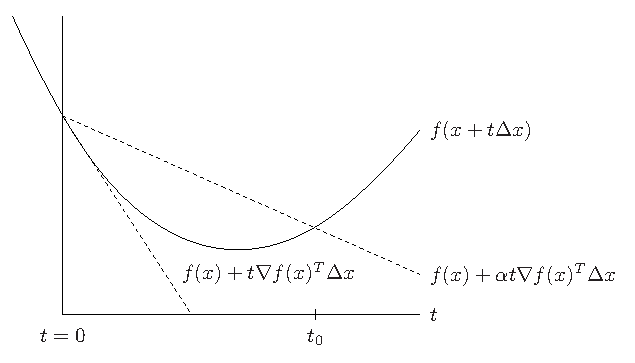
\includegraphics[width=.8\linewidth]{figures/ch09-fig01.pdf}
\caption*{图9.1\quad 回溯线搜索。曲线表示将 $f$ 限制在搜索直线上得到的函数。较低虚线为 $f$ 的线性外推，较高虚线的斜率缩小为其 $\alpha$ 倍。回溯条件要求 $f$ 位于较高虚线下方，即 $0\le t\le t_0$。}
\end{figure}
称为回溯，是因为线搜索从单位步长开始，每次将其乘 $\beta$ 缩小，直到满足停止条件 $f(x+t\Delta x)\le f(x)+\alpha t\nabla f(x)^\T\Delta x$。由于 $\Delta x$ 是下降方向，有 $\nabla f(x)^\T\Delta x<0$，所以 $t$ 足够小时，
\[
f(x+t\Delta x)\approx f(x)+t\nabla f(x)^\T\Delta x
<f(x)+\alpha t\nabla f(x)^\T\Delta x,
\]
这说明回溯线搜索最终会终止。常数 $\alpha$ 可理解为我们接受的函数减小量占线性外推所预测减小量的比例。（要求 $\alpha<0.5$ 的原因稍后会清楚。）

图9.1说明回溯条件。由图可见，而且可以证明，对 $t\ge0$，回溯退出不等式
$f(x+t\Delta x)\le f(x)+\alpha t\nabla f(x)^\T\Delta x$
在区间 $(0,t_0]$ 上成立。因此回溯会以满足
\[
t=1,\qquad\text{或}\qquad t\in(\beta t_0,t_0]
\]
的步长停止。第一种情况发生于 $t=1$ 满足回溯条件时，即 $1\le t_0$。特别地，回溯线搜索所得步长满足
\[
t\ge\min\{1,\beta t_0\}.
\]
当 $\dom f$ 不是整个 $\R^n$ 时，必须谨慎理解回溯中的条件
$f(x+t\Delta x)\le f(x)+\alpha t\nabla f(x)^\T\Delta x$。
按照函数在定义域之外取无穷大的约定，这个不等式蕴含 $x+t\Delta x\in\dom f$。实际实现时，先反复将 $t$ 乘 $\beta$，直到 $x+t\Delta x\in\dom f$。

% Source PDF page 480 (printed p. 466)
然后再开始检查 $f(x+t\Delta x)\le f(x)+\alpha t\nabla f(x)^\T\Delta x$ 是否成立。

参数 $\alpha$ 通常选在0.01至0.3之间，即接受的 $f$ 减小量为线性外推预测值的1\%至30\%。$\beta$ 常选在0.1（相当粗略的搜索）至0.8（较细的搜索）之间。

\section{梯度下降法}
搜索方向的自然选择是负梯度 $\Delta x=-\nabla f(x)$。所得算法称为\emph{梯度算法}或\emph{梯度下降法}。

\begin{origalgorithm}{9.3}
\emph{梯度下降法。}

给定初始点 $x\in\dom f$。

重复：
\begin{enumerate}
\item $\Delta x:=-\nabla f(x)$。
\item \emph{线搜索。}通过精确或回溯线搜索选择步长 $t$。
\item \emph{更新。}$x:=x+t\Delta x$。
\end{enumerate}
直到满足停止准则。
\end{origalgorithm}

停止准则通常为 $\norm{\nabla f(x)}_2\le\eta$，其中 $\eta$ 为很小的正数。多数实现中，在步骤1之后检查这一条件，而非在更新之后。

\subsection{收敛分析}
本节给出梯度法的简单收敛分析。以简洁记号 $x^+=x+t\Delta x$ 代替
$x^{(k+1)}=x^{(k)}+t^{(k)}\Delta x^{(k)}$，其中 $\Delta x=-\nabla f(x)$。假设 $f$ 在 $S$ 上强凸，因此存在正常数 $m,M$，使所有 $x\in S$ 满足 $mI\preceq\nabla^2f(x)\preceq MI$。定义 $\widetilde f:\R\to\R$ 为
$\widetilde f(t)=f(x-t\nabla f(x))$，即 $f$ 沿负梯度方向关于步长 $t$ 的函数。以下仅考虑满足 $x-t\nabla f(x)\in S$ 的 $t$。在（9.13）中取 $y=x-t\nabla f(x)$，得到 $\widetilde f$ 的二次上界：
\begin{equation}
\widetilde f(t)\le f(x)-t\norm{\nabla f(x)}_2^2
+\frac{Mt^2}{2}\norm{\nabla f(x)}_2^2.\tag{9.17}
\end{equation}

\subsubsection*{精确线搜索的分析}
假设使用精确线搜索，在（9.17）两边对 $t$ 最小化。左端得到 $\widetilde f(t_{\mathrm{exact}})$，其中 $t_{\mathrm{exact}}$ 是
